\section{Разработка алгоритма генерации расписания}

Для автоматического создания расписания будет использоваться метаэвристический подход, комбинирующий в себе сразу несколько алгоритмов.

Сперва будет получено первичное приемлемое решение --- то есть решение, удовлетворяющее минимальным (жёстким) требованиям. Допустимым решением для поставленной задачи будет являться расписание, содержащее в себе все дисциплины согласно учебному плану и не нарушающее никакие нормативы.

Далее итеративным методом расписание будет оцениваться и улучшаться путём перестановки различных учебных занятий местами.

\subsection{Минимальные требования к расписанию}

В этой главе будут рассмотрены строгие требования к расписанию работы учебного заведения. Расписание на семестр должно строго соответствовать учебному плану и количеству часов лекций, семинаров и лабораторных занятий. При этом нельзя просто «запихнуть» по 10 учебных занятий в каждый день, существуют нормативы времени по нагрузке как на преподавателей, так и на студентов. Также нельзя забывать и о рабочих часах самого учебного заведения, пары должны начинаться в строго отведённое под них время с 8:30 утра, по 22:50, без учёта выходных дней и праздников. Список нерабочих праздничных дней задаётся «Трудовым кодексом Российской Федерации» от 30.12.2001 №~197-ФЗ (ред. от 14.02.2024) \cite{tkrf:112}. Упрощённая диаграмма документов и таблиц управления учебным процессом приведена на рисунке ниже (см. \figref{fig:docs}).

\begin{figure}[H]
	\centering
	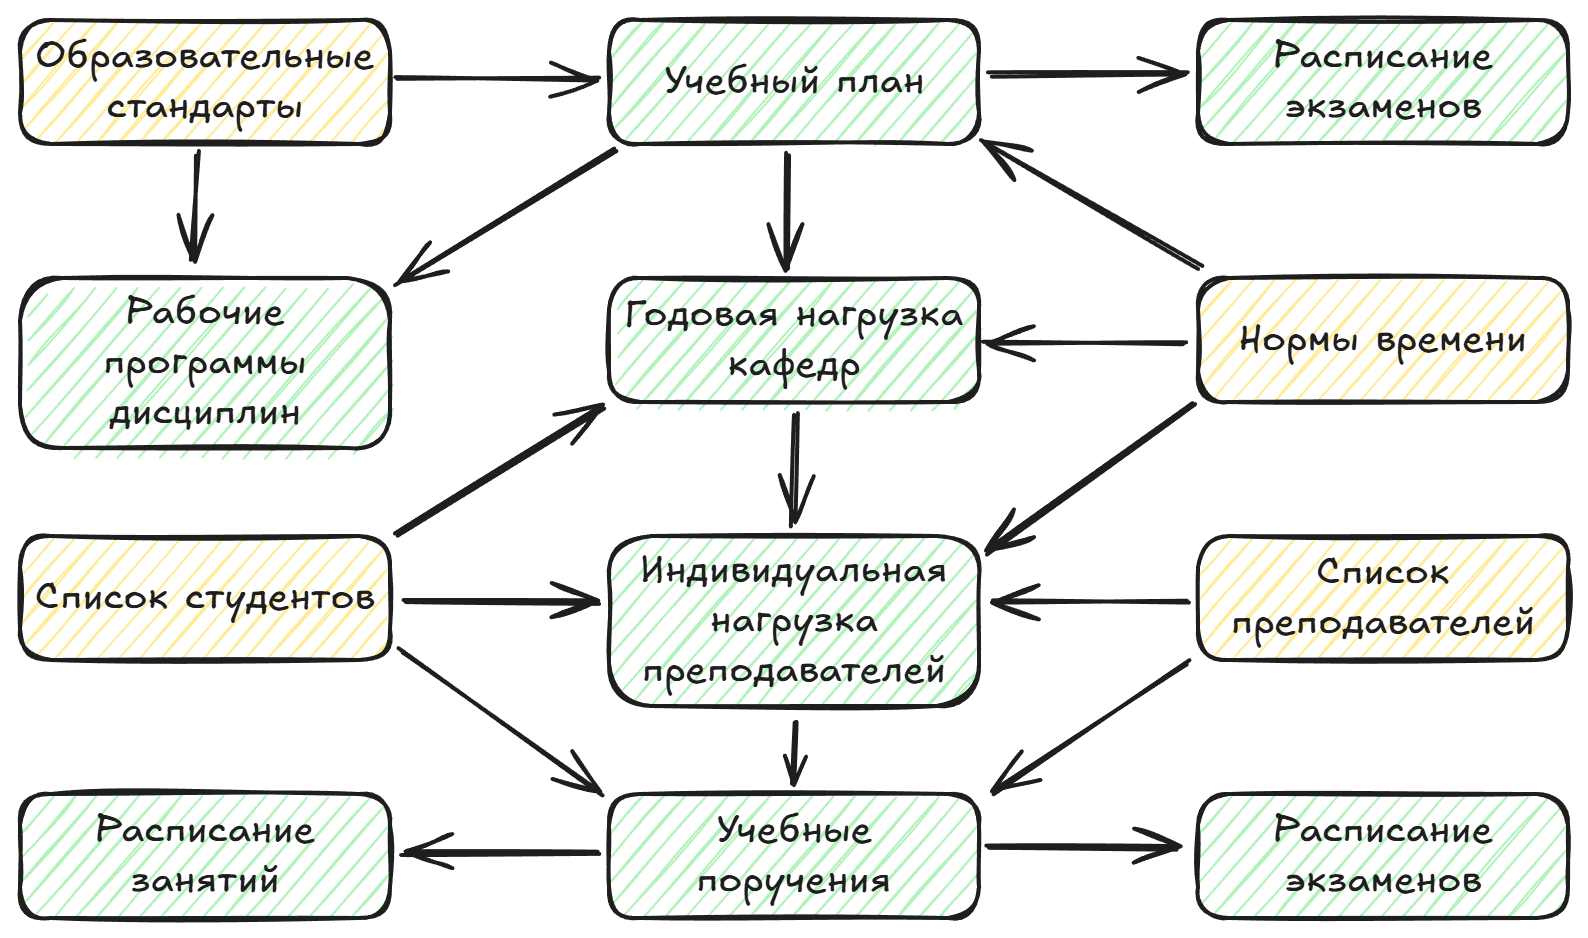
\includegraphics[width=1\textwidth]{images/ch2/docs.png}
	\caption{Диаграмма документов и таблиц управления учебным процессом}
	\label{fig:docs}
\end{figure}

Список студентов будет делиться на направления, согласно учебным планам, а также на группы и подгруппы для проведения семинаров и лабораторных занятий соответственно. Следует подметить, что деление на подгруппы является рудиментарным процессом, изначальный смысл которого заключался в невозможности вместить достаточное количество студентов в классы с компьютерами.

Не менее важным является подбор аудиторий для проведения учебных занятий. Главным параметром каждой аудитории является вместимость --- нельзя назначать учебное занятие в аудиторию, которая физически не может вместить весь контингент студентов и преподавателей на данное учебное занятие. Дополнительным, не менее важным параметром является требуемое оборудование для проведения учебного занятия: мультимедийное и лабораторное оборудование.

Схематичное дробление контингента студентов и здания вуза предоставлено на рисунке ниже (см. \figref{fig:fragmentation}).

\begin{figure}[H]
	\centering
	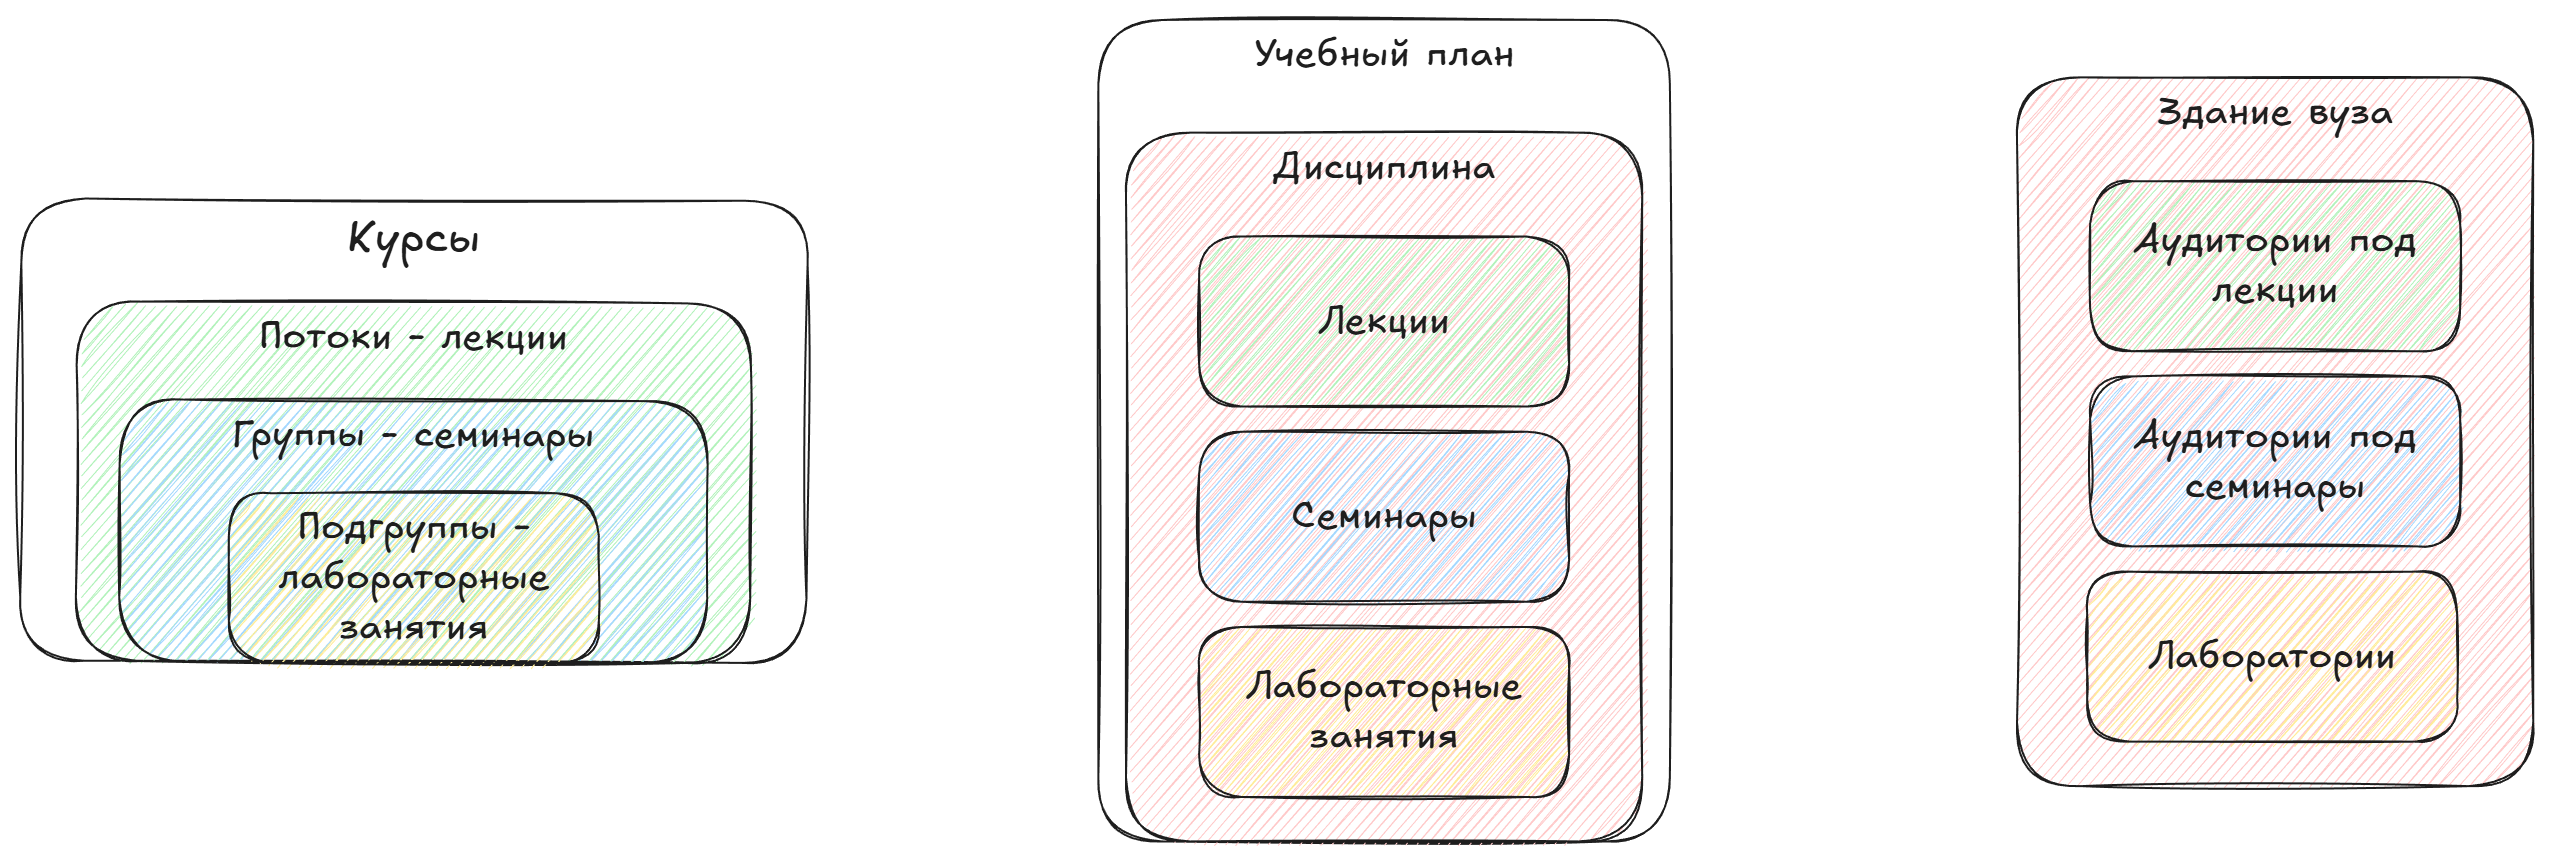
\includegraphics[width=1\textwidth]{images/ch2/fragmentation.png}
	\caption{Схематичное дробление контингента и здания вуза}
	\label{fig:fragmentation}
\end{figure}

\subsection{Допустимое решение}

\subsubsection{Коллапс волновой функции}

 WFC \cite{alonecoder:wavecollapse}, вдохновлённый редукцией фон Неймана. Название алгоритма произошло от физического процесса, при котором волновая функция, описывающая вероятностное состояние квантовой системы, при измерении переходит из суперпозиции возможных состояний в одной конкретное наблюдаемое состояние.

 В контексте задачи с составлением расписания её можно представить как суперпозицию здания университета. В каждой аудитории на каждый момент времени семестра существуют все возможные (удовлетворяющие ограничениям) учебные занятия конкретных групп и студентов. Для каждой такой ячейки высчитывается мера неопределённости --- энтропия, то есть количество возможных состояний. Далее ячейки с наименьшей энтропией коллапсируют в конкретные состояния из набора возможных, при этом учитывается вес состояния. Весом выступает функция полезности, как например большие веса в начале дня для групп на дневном обучении, и наоборот для групп на вечернем обучении. Именно гибкость этой функции позволяет модифицировать алгоритм решения под конкретные особенности того или иного образовательного учреждения. Коллапс волновой функции позволит найти приемлемое решение, то есть то, которое соответствует всем ограничениям, но в силу своей вероятностной природы решение не гарантирует глобального оптимума. Для того чтобы приблизить решение к глобальному оптимуму потребуется дополнительный шаг --- генетический алгоритм.

 \paragraph{Разрешение противоречий в WFC}

 Если в какой-то момент у всех доступных ячеек не остаётся допустимых вариантов коллапса, возникает противоречие.

 Для решения таких ситуаций в работе рассматриваются четыре подхода:
 \begin{itemize}
 	\item backtracking;
 	\item backjumping;
 	\item block based method;
 	\item полный перезапуск с нуля.
 \end{itemize}

 Backtracking. Метод backtracking является классическим способом устранения противоречий в задачах поиска с ограничениями.
 Если после очередного выбора система приходит к неразрешимому состоянию, алгоритм возвращается к предыдущему шагу, отменяет последнее решение и пробует следующий вариант.

 Формально процесс можно описать последовательностью решений \formref{eq:backtrack-seq}:
 \begin{equation}
 	S = \{s_1, s_2, \dots, s_k\},
 	\label{eq:backtrack-seq}
 \end{equation}
 \formwhere{где $S$~--- последовательность принятых решений;
 	\formwherenext{$s_i$}{решение на шаге $i$};
 	\formwherenext{$k$}{номер текущего шага}.}
 Каждое решение влияет на множество допустимых значений для следующих ячеек.
 При обнаружении противоречия выполняется откат \formref{eq:backtrack-rollback}:
 \begin{equation}
 	S \leftarrow \{s_1, s_2, \dots, s_{k-1}\}.
 	\label{eq:backtrack-rollback}
 \end{equation}
 \formwhere{где $\leftarrow$~--- возврат к предыдущему состоянию последовательности;
 	\formwherenext{$k-1$}{индекс шага, на который выполняется откат}.}

 Преимущество backtracking заключается в том, что он позволяет сохранить уже построенную часть расписания и использовать её повторно.
 Это особенно важно в задачах, где большая часть размещённых занятий остаётся корректной, а конфликт возникает только в локальной области.

 Однако у метода есть существенный недостаток: при большом числе ограничений количество возвратов может быстро расти.
 В задаче составления расписания это означает, что алгоритм может многократно пересчитывать одни и те же фрагменты, особенно если противоречие вызвано неудачным ранним выбором.

 Backjumping. Backjumping является расширением backtracking.
 Вместо возврата к непосредственно предыдущему решению алгоритм анализирует причину противоречия и откатывается не на один шаг, а к наиболее раннему решению, которое действительно повлияло на возникновение ошибки.

 Идея метода особенно полезна в расписаниях, где конфликт часто связан не с последним назначением, а с более ранним выбором, например:
 \begin{itemize}
 	\item преподаватель уже оказался занят в нужное время;
 	\item аудитория была закреплена за другим занятием;
 	\item группа получила пересечение по нескольким предметам.
 \end{itemize}

 Если конфликт возник из-за решений $s_i, s_j, s_k$, то backjumping позволяет перейти не к $s_{k-1}$, а сразу к наиболее релевантному из них.
 Это сокращает число бесполезных откатов и уменьшает время поиска.

 В практическом применении к расписанию метод backjumping полезен тогда, когда система хранит информацию о причинах исключения вариантов.
 Например, при удалении варианта можно фиксировать, какие уже назначенные занятия сделали его невозможным.
 Тогда при противоречии можно определить, какой именно шаг следует пересмотреть.

 Недостаток метода состоит в том, что для его эффективной работы требуется дополнительный учёт причин конфликтов, а это усложняет реализацию.

 Block based method. Block based method основан на локализации проблемы внутри части пространства поиска.
 Вместо пересчёта всей модели алгоритм выделяет блок --- набор связанных ячеек, внутри которого возникло противоречие, и пытается восстановить только этот фрагмент.

 Для задачи расписания блоком может быть:
 \begin{itemize}
 	\item одна учебная неделя;
 	\item один день;
 	\item конкретная пара групп, преподавателей и аудиторий.
 \end{itemize}

 Преимущество такого подхода состоит в том, что большая часть уже построенного расписания сохраняется.
 Это особенно удобно, если противоречие локализуется в ограниченной области и не затрагивает всю структуру решения.

 Принцип работы можно описать следующим образом:
 \begin{enumerate}
 	\item выделяется блок, в котором обнаружено противоречие;
 	\item внутри блока восстанавливается множество допустимых вариантов;
 	\item выполняется повторный коллапс только для этого блока;
 	\item если блок снова приводит к конфликту, он расширяется или пересобирается заново.
 \end{enumerate}

 В рамках расписания такой подход уменьшает число глобальных перезапусков, но требует аккуратного определения границ блока.
 Если блок выбран слишком маленьким, противоречие может просто переместиться в соседнюю область; если слишком большим --- метод теряет локальные преимущества.

 Начать всё заново. Подход полного перезапуска предполагает, что при обнаружении тупика алгоритм сбрасывает текущее состояние и строит решение заново.
 В WFC это означает удаление всей текущей частичной раскладки и повторный запуск процесса коллапса с новыми случайными выборами.

 Для задачи составления расписания такой подход особенно оправдан, потому что качественное решение часто зависит от ранних случайных выборов.
 Если эти выборы оказались неудачными, дальнейшее локальное исправление может быть неэффективным.
 В этом случае проще и быстрее полностью перезапустить алгоритм и получить новую траекторию поиска.

Именно этот подход был выбран в реализации алгоритма WFC для генерации расписания ВУЗа, так как он является очень простым в реализации и на удивление эффективным.

 \subsubsection{Satisfiability solvers}

 Satisfiability solvers (SAT solvers) --- это программы, решающие задачи булевой выполнимости
 (Boolean Satisfiability Problem).

 Основным вопросом SAT-задачи является: «можно ли подобрать значения true/false для переменных так, чтобы логическое выражение стало истинным?»

 Например, задана булева формула \formref{eq:sat-formula}:
 \begin{equation}
 	(A \lor B) \land (\neg A \lor C)
 	\label{eq:sat-formula}
 \end{equation}
 \formwhere{где $A$, $B$, $C$~--- булевы переменные.}

 SAT solver пытается найти такие значения переменных \formref{eq:sat-values}:
 \begin{equation}
 	A = \mathrm{false},\quad B = \mathrm{true},\quad C = \mathrm{true}
 	\label{eq:sat-values}
 \end{equation}
 \formwhere{где $\mathrm{false}$ и $\mathrm{true}$~--- логические значения «ложь» и «истина».}

 при которых вся формула становится истинной.

 Если такого набора не существует, solver доказывает, что формула
 невыполнима.

 \paragraph{Satisfiability Modulo Theories}

 Классический SAT solver работает только с булевой логикой, однако реальные задачи часто требуют работы с числами, массивами, строками и битовыми операциями.

 Для этого используются SMT solver'ы (Satisfiability Modulo Theories) \cite{z3:github}.

 Например, SMT solver способен анализировать систему ограничений \formref{eq:smt-x}--\formref{eq:smt-y-max}:
 \begin{equation}
 	x > 10
 	\label{eq:smt-x}
 \end{equation}
 \begin{equation}
 	y = x + 2
 	\label{eq:smt-y-def}
 \end{equation}
 \begin{equation}
 	y < 5
 	\label{eq:smt-y-max}
 \end{equation}
 \formwhere{где $x$, $y$~--- целочисленные переменные;
 	\formwherenext{$10$, $2$, $5$}{числовые константы в ограничениях}.}

 и определить, что такая система противоречива.

 \paragraph{Принцип работы}

 SAT/SMT solver --- это механизм поиска значений, удовлетворяющих набору ограничений.

 Вместо ручного перебора вариантов программист описывает:

 \begin{itemize}
 	\item переменные;
 	\item ограничения;
 	\item условия задачи.
 \end{itemize}

 После этого solver самостоятельно ищет решение или доказывает, что решения не существует. Такая программа может быть полезной при формировании учебных планов, чтобы удостовериться, что план не будет нарушать жёсткие ограничения.

 SMT-solver также может выступать в роли алгоритма формирования приемлемого решения, однако его природа заключается в том, чтобы найти любое решение но быстро. WFC же в то время сможет не просто найти случайное решение, но и уже на этом этапе применить ряд оптимизаций решения.

\subsection{Оценка решения}

После получения первичного решения, которое удовлетворяет всем обязательным требованиям требуется провести итеративный процесс улучшения этого расписания. Для того, чтобы что-либо улучшать, нужно уметь давать оценку полученным результатам.

Самым важным критерием оценки является соответствие минимальным требованиям:

\begin{itemize}
	\item все учебные занятия согласно учебному плану \cite{stankin:edu_programs};
	\item весь учебный процесс проходит в период согласно календарному учебному графику \cite{stankin:calendar};
	\item не нарушаются нормы времени;
	\item учебные занятия должны начинаться в строго отведённое под них время с 8:30 утра, по 22:50, без учёта выходных дней и праздников \cite{tkrf:112}.
\end{itemize}

Для оценки будет рассчитываться множество различных параметров. Одним из самых главных таких параметров является непрерывность расписания --- в прекрасном расписании будущего не должно быть «окон», на которых студенты имеют свойство расходится по домам.

Ещё один важный параметр --- это равномерность расписания. Не должно быть расписания, где в понедельник пять пар, а во вторник только одна. Согласно исследованию, проведённому Клеванским Николаем Николаевичем \cite{klivansky:forming_schedule} студенты предпочитают, когда одни и те же пары проводятся в одно и то же время в разные дни недели. Соответственно существует три оценки равномерности:

\begin{itemize}
	\item равномерность загруженности;
	\item равномерность начала занятий;
	\item равномерность идентичности пар по дням / неделям.
\end{itemize}

Дополнительным параметром может являться «компоновка» ВУЗа. Для экономии временных и финансовых ресурсов можно попробовать уместить весь учебный процесс в меньший набор аудиторий. Также можно пробовать уменьшать среднюю дистанцию, требуемую для перехода из одной аудитории в другую между учебными занятиями. В случае проведения лабораторных занятий дистанционно можно не делить на подгруппы, начинать семинары только после лекций по каждой дисциплине и т. д.

\subsection{Оптимизация решения}

\subsubsection{Генетический алгоритм}

Генетический алгоритм представляет собой эвристический метод поиска оптимального решения,
механизм работы которого аналогичен процессу естественного отбора в природе. В рамках данной задачи
в качестве генома рассматривается полное расписание учебного заведения на семестр.

В научной литературе уже были упомянуты комбинации алгоритма WFC с генетическим алгоритмом \cite{bailly:geneticwfc}, однако этот подход не применялся к задачам составления расписания.

Хромосома кодирует расписание на один семестр и состоит из набора генов, где каждый ген
соответствует конкретному элементу расписания.
Размер хромосомы определяется \formref{eq:chromosome-size}:
\begin{equation}
	|H| = n \times 6 \times 182{,}625,
	\label{eq:chromosome-size}
\end{equation}
\formwhere{где $|H|$~--- размер хромосомы;
	\formwherenext{$n$}{количество учебных групп};
	\formwherenext{$6$}{количество учебных дней в неделю};
	\formwherenext{$182{,}625$}{усреднённое количество учебных дней в семестре (варьируется каждый семестр)}.}

Операторы мутации реализуются с использованием локальных методов поиска, например алгоритма имитации отжига, что позволяет эффективно исследовать окрестность текущего решения и избегать застревания в локальных минимумах.

\subsubsection{Имитация отжига}

Имитация отжига (SA) представляет собой стохастический метод локального поиска, основанный на аналогии с физическим процессом охлаждения твёрдых тел, при котором система постепенно переходит к состоянию с минимальной энергией. В контексте задачи оптимизации расписания данный алгоритм используется для улучшения текущего решения путём итерационного поиска его окрестностей (см. \figref{fig:sa}).

\begin{figure}[H]
	\centering
	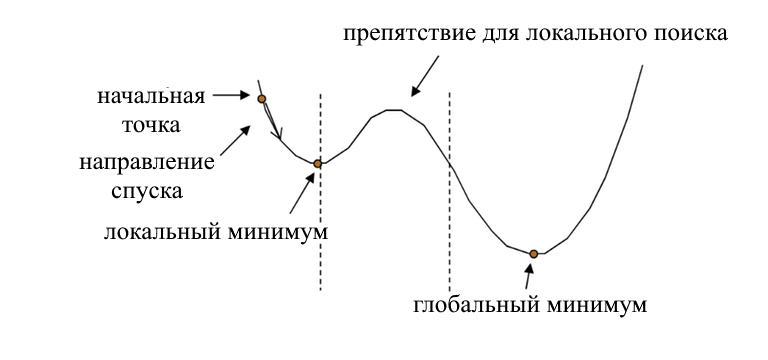
\includegraphics[width=0.9\textwidth]{images/ch2/sa.png}
	\caption{Проблематика локальных методов поиска}
	\label{fig:sa}
\end{figure}

На каждой итерации из текущего решения формируется новое, соседнее решение путём небольшого случайного
изменения (например, перестановки занятий в расписании). Если новое решение имеет более высокое значение целевой функции, оно принимается. В противном случае оно может быть принято с некоторой вероятностью, определяемой \formref{eq:sa-accept}:
\begin{equation}
	P = \exp\left(-\frac{\Delta E}{T}\right),
	\label{eq:sa-accept}
\end{equation}
\formwhere{где $P$~--- вероятность принятия ухудшающего решения;
	\formwherenext{$T$}{параметр температуры алгоритма};
	\formwherenext{$\Delta E$}{ухудшение значения функции приспособленности}.}

Параметр температуры постепенно уменьшается согласно заданному расписанию охлаждения, что приводит к снижению вероятности принятия ухудшающих решений и обеспечивает сходимость алгоритма к локально оптимальному решению.

\subsection{Вывод по второй главе}

Предложенный гибридный подход, основанный на применении алгоритма коллапса волновой
функции и последующей оптимизации с помощью генетического алгоритма, позволяют решать задачу
составления расписания, при этом поддерживая достаточную гибкость для адаптации к различным
образовательным учреждениям.
